% Laborationsmall.tex
\documentclass[a4paper]{article}

\usepackage[swedish]{babel}
\usepackage[utf8x]{inputenc}

\usepackage{multicol}
\usepackage[vmargin=3cm,hmargin=2cm]{geometry}
\usepackage{parskip}
\usepackage[runin]{abstract}
\renewcommand{\abstitleskip}{0mm}

\usepackage{hyperref}
\usepackage{amsmath}
\usepackage{lmodern}
\usepackage[T1]{fontenc}
\usepackage{pgfplots}
\pgfplotsset{compat=1.13}
\usetikzlibrary{decorations.pathreplacing}
\usetikzlibrary{arrows.meta}
\usepackage{placeins}
\usepackage{siunitx}
\usepackage[numbered,framed]{matlab-prettifier}

\lstset{
	style              = Matlab-editor,
	basicstyle         = \mlttfamily,
	mlshowsectionrules = true,
}

\addto\extrasswedish{%
	\def\equationautorefname{Ekvation}%
	\def\figureautorefname{Figur}%
	\def\tableautorefname{Tabell}%
	\def\sectionautorefname{Rubrik}%
	\def\subsectionautorefname{Underrubrik}%
	\def\pageautorefname{Sida}%
}

\usepackage{graphicx}
%\usepackage{subcaption}
\usepackage{ccaption}
\captionnamefont{\it}
\captiontitlefont{\it}

% Hack för att få komma istället för punkt i matematiska uttryck
% $3.141592$ blir 3,141592
% Om man använder komma direkt får man ett litet oönskat mellanrum:
% $3,141592$ blir 3, 141592
\DeclareMathSymbol{,}{\mathpunct}{letters}{"3B}
\DeclareMathSymbol{.}{\mathord}{letters}{"3B}
\DeclareMathSymbol{\decimal}{\mathord}{letters}{"3A}

% Kommando för att få icke-kursiva enheter i matematiska uttryck
% $10\unit{km}$ blir 10 km
\newcommand{\unit}[1]{\ensuremath{\,\mathrm{#1}}}

\usepackage{lastpage}
\usepackage{fancyhdr}
\pagestyle{fancy}
\fancyhf[C]{\thepage}
\fancyhead[C]{Våglära och optik, FAFF30}
\fancyhead[R,L]{}
\fancypagestyle{plain}{
  \fancyhead{}
}
%\setcounter{secnumdepth}{-1} % Stänger av numrering.

\title{Laborationen ”Ljusets diffraktion”}
\author{Johan Boström\\Anton Johansson\\Lunds Universitet}

\makeatletter
%\renewcommand{\section}{\@startsection
%{section}%                   % the name
%{1}%                         % the level
%{0mm}%                       % the indent
%{-\baselineskip}%            % the before skip
%{0.5mm}%          % the after skip
%{\normalfont\bfseries}} % the style
%\renewcommand{\sectionmark}[1]{ }
%\renewcommand{\thesection}{}

\renewcommand*\maketitle{
  {
    \begin{center}
      {\huge\bfseries \@title}\\
      \vspace{5mm}
      {\large \@author}
    \end{center}
    \vspace{2mm}
  }
}
\makeatother

\begin{document}
\maketitle

\renewcommand{\abstractname}{Abstract} % Om vi vill ha titeln till abstracten på engelska.

\begin{abstract}
  %Kort beskrivning  av resultaten (5-10  rader). Det ska inte  vara en innehållsbeskrivning (först gör vi det, sen använder vi den metoden, och så jämför vi det med de där tidigare kända resultaten, etc) utan vara   koncentrerat  till   ”resultatet”,   vad   man  kommer fram till. Sammanfattningen är uppsatsens löpsedel. Den ska vara kort och kärnfull och locka läsare genom att  effektivt göra klart vad det är man uppnår genom att läsa rapporten.
  
\end{abstract}

\vspace{2mm}

\hspace{-3mm}
\begin{tabular}{ll}
Laborationen genomförd: &	2017-05-04 \\
%Rapporten kamratgranskad: &	2013-xx-xx \\
Lämnad till handledare: &	2017-xx-xx \\
\end{tabular}

\vspace{3mm}

\section{Inledning}
  %Preliminär beskrivning av uppgiften  i lättfattliga termer. Bakgrunden till att man intresserar sig för detta problem, denna uppgift. Hur den ingår i ett större sammanhang.

%  En detaljerad beskrivning av vad det hela går ut på, och vad exakt din uppgift   i    sammanhanget   är.    Utrustningsförutsättningar.   Det
%  ursprungligen avsedda målet. Även den i ämnet oinsatte ska ha en ärlig
%  chans att förstå de stora dragen.
%
%  Beskrivning av hur rapporten är uppbyggd, för att göra det möjligt för
%  läsaren att förstå vad som  pågår, ge läsaren rätta förväntningar, och
%  för  att  underlätta direktåtkomst  av  för  den individuelle  läsaren
%  särskilt intressanta delar.

\section{Teori}

\subsection{Diffraktion}

\FloatBarrier

\pgfmathsetmacro{\numSources}{4}
\pgfmathsetmacro{\numWaves}{10}
\pgfmathsetmacro{\numIncoming}{8}
\pgfmathsetmacro{\wavesDist}{0.25}

När en våg passerar en spalt eller ett annat objekt som blockerar ljuset i vissa områden kommer den enligt Huygens princip att uppföra sig som om det funnits en mängd punktkällor utspridda över hela ytan där objektet är genomskinligt. Vågorna som bildas från dessa kommer därefter att interferera med varandra. Detta demonstreras i \autoref{fig:singleInterference} med kollimerat infallande ljus approximerat med endast \numSources~punktkällor.

\begin{figure}[ht]
	\centering
	\begin{tikzpicture}
	\draw[line width=0.75mm] (0, {1 + \wavesDist*\numWaves}) -- (0, 0.5); % Draw the top half of the slit.
	\draw (0, 0.5) -- (0, -0.5); % Draw the wavefront inside the slit.
	\draw[line width=0.75mm] (0, -0.5) -- (0, {-1 - \wavesDist*\numWaves}); % Draw the lower half of the slit.
	\foreach \incoming in {1,...,\numIncoming} % Draw all incoming wavefronts.
	{
		\draw ({-\incoming*\wavesDist}, {-0.5 - \wavesDist*\numWaves}) -- ({-\incoming*\wavesDist}, {0.5 + \wavesDist*\numWaves});
	}
	\foreach \source in {1,...,\numSources} % For each source
	{
		\node[circle,fill=black,inner sep=0,minimum size=5] at (0, {(\source-1)/(\numSources-1) - 0.5}) {}; % Draw the source
		\foreach \waveIdx in {1,...,\numWaves}
		{ % and numWaves waves spaced with wavesDist
			\draw (0, {(\source-1)/(\numSources-1) - 0.5 - \wavesDist*\waveIdx}) arc [radius={\wavesDist*\waveIdx}, start angle=-90, end angle=90];
		}
	}
	\end{tikzpicture}
	\caption{Demonstration av diffraktion i enkelspalt då vågorna infaller från vänster. Där vågorna överlappar interfererar de konstruktivt, medan det är svårare att se när de interfererar destruktivt. Förutom huvudmaximat rakt åt höger syns även ett ytterliggare maximum i vardera riktningen. I en riktig spalt blir det oändligt många punktkällor som måste adderas ihop i en integral.}
	\label{fig:singleInterference}
\end{figure}

För att summera bidragen från de oändligt många punktkällorna används Fresnel-Kirchhoffs integral \cite[p.~330]{pearsonIntroOpt}

\begin{equation}
	E_P = \frac{-i k E_S}{2\pi} e^{-i \omega t} \iint\limits_{\mathrm{Objektet}} {F(\theta)\frac{e^{i k (r + r')}}{r r'} d A}
	\label{eq:frKirInt}
\end{equation}

där $E_P$ är det elektriska fältet på skärmen med avstånder $r$ från den infinitesimala arean $d A$ på objektet. På samma sätt är $E_S$ det elektriska fältet av punktkällan och $r'$ dess avstånd till $d A$. $k$ är vågtalet, $\omega$ är vinkelfrekvensen och $F(\theta) = \frac{1 + \cos\theta}{2}$ är en obliquity-faktor som är nära ett då vågen passerar rakt igenom objektet men avtar för högra vinklar.

\subsubsection{Fraunhoferdiffraktion}

När både källan och skärmen är långt borta från objektet varierar både $r$ och $r'$ i \eqref{eq:frKirInt} mycket lite över objektets area och kan flyttas ut ur integralen. Samtidigt blir obliquity-faktorn nästan konstant då $\theta$ är nära noll och även den kan tas ut ur integralen. Integralen kan då förenklas till \cite[p.~331]{pearsonIntroOpt}

\begin{equation}
	E_P = C_0 e^{-i \omega t} \iint\limits_{\mathrm{Objektet}} {e^{i k r} dA}
	\label{eq:fraunhofer}
\end{equation}

där $C_0$ är en konstant. Om positionen på skärmen betecknas med ortsvektorn $\boldsymbol{p}$ och positionen på objektet med $\boldsymbol{p'}$ blir

\begin{equation}
	r = \sqrt{(\boldsymbol{p} - \boldsymbol{p'})\cdot(\boldsymbol{p} - \boldsymbol{p'})} = \sqrt{\boldsymbol{p}\cdot\boldsymbol{p} - 2 \boldsymbol{p}\cdot\boldsymbol{p'} + \boldsymbol{p'}\cdot\boldsymbol{p'}}\text{.}
\end{equation}

Man kan nu bryta ut $|\boldsymbol{p}|$

\begin{equation}
r = |\boldsymbol{p}|\sqrt{1 - \frac{2\boldsymbol{p}\cdot\boldsymbol{p'}}{|\boldsymbol{p}|^2} + \left(\frac{|\boldsymbol{p'}|}{|\boldsymbol{p}|}\right)^2}
\end{equation}

och då $|\boldsymbol{p'}|\ll|\boldsymbol{p}|$ blir $\left(\frac{|\boldsymbol{p'}|}{|\boldsymbol{p}|}\right)^2\approx 0$ och man kan utveckla kvadratroten till

\begin{equation}
	r = |\boldsymbol{p}|\left( 1 - \frac{\boldsymbol{p}\cdot\boldsymbol{p'}}{|\boldsymbol{p}|^2} \right) = |\boldsymbol{p}| - \left(\frac{\boldsymbol{p}}{|\boldsymbol{p}|}\right)\cdot\boldsymbol{p'}\text{.}
\end{equation}

Här är $|\boldsymbol{p}|$ konstant i integralen i \eqref{eq:fraunhofer} och kan absorberas i konstanten. Med beteckningen $\boldsymbol{k} = k \frac{\boldsymbol{p}}{|\boldsymbol{p}|}$ kan \eqref{eq:fraunhofer} skrivas

\begin{equation}
	E_P = C_1 e^{-i \omega t} \iint\limits_{\mathrm{Objektet}} {e^{-i \boldsymbol{k}\cdot\boldsymbol{p'}} dA}\text{.}
\end{equation}

Nu är integralen exakt definitionen av en tvådimensionell Fouriertransform av en funktion som är ett där objektet släpper igenom ljus och noll där den inte gör det.

\subsubsection{Fresneldiffraktion}

Då man inte kan göra de approximationer som leder fram till Fraunhoferdiffraktion måste man lösa \eqref{eq:frKirInt} direkt, vilket bara går analytiskt för ett fåtal specialfall. Två sådana specialfall behandlas i \cite{pearsonIntroOpt}: objekt med cirkulär samt rektangulär symmetri. Ytterliggare beräknas integralen för en rektangulär öppning då variationerna av obliquity-faktorn och produkten $r r'$ försummas.

\pgfmathsetmacro{\numFresnelWaves}{8}
\pgfmathsetmacro{\fresnelWavesDist}{0.1}
\pgfmathsetmacro{\leftRightDist}{2.25}

\begin{figure}[ht]
	\centering
	\begin{tikzpicture}[scale=2]
	
	\node[circle,fill=black,inner sep=0,minimum size=3] at (0,0) {}; % Draw the source
	\foreach \waveIdx in {1,...,\numFresnelWaves}
	{ % and numFresnelWaves waves spaced with fresnelWavesDist
		\draw (0, {-\fresnelWavesDist*\waveIdx}) arc [radius={\fresnelWavesDist*\waveIdx}, start angle=-90, end angle=90]; % Waves move to the right +-90*.
		%\draw ({\fresnelWavesDist*\waveIdx/sqrt(2)}, {-\fresnelWavesDist*\waveIdx/sqrt(2)}) arc [radius={\fresnelWavesDist*\waveIdx}, start angle=-45, end angle=45]; % Waves move to the right +-45*.
	}
	
	% Draw the slit so that it covers 45* of the source's view.
	\draw[line width=0.75mm] ({\fresnelWavesDist*\numFresnelWaves/sqrt(2)}, {1.4*\fresnelWavesDist*\numFresnelWaves}) -- ({\fresnelWavesDist*\numFresnelWaves/sqrt(2)}, {\fresnelWavesDist*\numFresnelWaves/sqrt(2)}); % top half
	\draw[line width=0.25mm,red] ({\fresnelWavesDist*\numFresnelWaves/sqrt(2)}, {\fresnelWavesDist*\numFresnelWaves/sqrt(2)}) -- ({\fresnelWavesDist*\numFresnelWaves/sqrt(2)}, {-\fresnelWavesDist*\numFresnelWaves/sqrt(2)}); % emphasis on the aperture.
	\draw[line width=0.75mm] ({\fresnelWavesDist*\numFresnelWaves/sqrt(2)}, {-\fresnelWavesDist*\numFresnelWaves/sqrt(2)}) --({\fresnelWavesDist*\numFresnelWaves/sqrt(2)}, {-1.4*\fresnelWavesDist*\numFresnelWaves}); % lower half

	\pgfmathsetmacro{\Start}{ceil(\numFresnelWaves/sqrt(2))} % Only the last few wavefronts actually reach the aperture.
	\foreach \waveIdx in {\Start,...,\numFresnelWaves} % For all those that do
	{
		\pgfmathsetmacro{\R}{\fresnelWavesDist*sqrt(\waveIdx*\waveIdx - \numFresnelWaves*\numFresnelWaves/2)} % Calculate the radius of the wavefront at the aperture.
		\draw[dashed] ({\fresnelWavesDist*\numFresnelWaves/sqrt(2)}, {\R}) -- ({\leftRightDist*\fresnelWavesDist*\numFresnelWaves}, {\R}); % Connect the two images (upper line)
		\draw[dashed] ({\fresnelWavesDist*\numFresnelWaves/sqrt(2)}, {-\R}) -- ({\leftRightDist*\fresnelWavesDist*\numFresnelWaves}, {-\R}); % Connect the two images (lower line)
		\draw[red] ({\leftRightDist*\fresnelWavesDist*\numFresnelWaves}, 0) circle ({\R)}); % Draw the intersections of the wavefronts with the aperture.
	}
	
	\end{tikzpicture}
	\caption{Illustration av hur fresnelzoner uppkommer i en cirkulär öppning. Till vänster visas hur vågfronterna når öppningen efter olika lång sträcka och därmed olika fas. Till höger visas var vågfronterna skär den cirkulära öppningen, varje cirkel är då i fas. I Fraunhoferdiffraktion är ljuskällan så långt bort att alla vågfronterna når öppningen samtidigt utan fasskillnad.}
	\label{fig:fresnelZones}
\end{figure}

\FloatBarrier

% Cirkulära vågfronter, analogi med lök?

\section{Metod}
  % De  olika  stegen  i  uppgiftens genomförande.  Till  exempel  val  av
  % algoritmer,  programspråk och  annan programvara,  undersökningsmetod,
  % statistiska  metoder. Där  valmöjligheter finns,  diskutera de  gjorda
  % valen.
  
  En laserstråle linjerades och kollimerades och riktades mot en skärm. Bakom skärmen placerades en kamera som kopplades in till ett program på en dator. En hållare som till exempel kan innehålla olika spaltsystem placerades på lämpligt avstånd från skärmen så att alla mönster blev av rimliga storlekar.
  För att mäta detta avstånd användes en dubbelspalt med kända mått och intensitetsfördelningen passades in på en teoretiskt beräknad kurva i programmet. Sedan placerades i tur och ordning en enkelspalt, en tråd, ett flerspaltsystem och en ställbar spalt på samma avstånd från skärmen och intensitetsfördelningarna mättes. Intensitetsfördelningarna passades sedan in över teoretiska intensitetsfördelningar så att relevanta parametrar kunde beräknas.
  
  Sedan togs utrustningen som kollimerade laserstrålen bort och den divergerande strålen läts belysa en cirkel, en ställbar spalt samt en egg. Diffraktionsmöstren fotograferades och för den ställbara spalten filmades förändringarna då spaltbredden förändrades.
  
  \subsection{Datorsimulering}
  
  För att kunna jämföra med vad teorin förutsäger skrevs ett antal skript i matlab som skulle simulera Fraunhofer- och Fresneldiffraktion. Fraunhoferdiffraktionen implementerades med hjälp av matlabs inbyggda FFT algoritm \lstinline{fft2} och Fresneldiffraktion implementerades för specialfallet med en egg genom funktionerna  \lstinline{fresnelc} och \lstinline{fresnels}.
  
  \begin{figure}[ht] % Exempel på matlab kod.
  \centering
  \begin{lstlisting}
function a = f(b)
	a = b .^ 2; % Matlab code example.
end
  \end{lstlisting}
  \end{figure}

\section{Resultat}

I alla mätningar användes ett CCD-chip med ett begränsat exponeringsintervall. Intensitetsdatan är därmed normaliserad mellan $0$ och $1$, där $1$ representerar den maximala intensiteten som kan mätas av chippet.

\subsection{Mätning av spaltsystem i Fraunhoferregimen}

I \autoref{fig:dubbelspalt} presenteras den uppmätta intensitetsfördelningen i Fraunhoferregimen för en dubbelspalt med spaltavståndet \SI{100}{\micro\m} och spaltbredden \SI{250}{\micro\m}. Figuren innehåller även det förväntade teoretiska resultatet som beräknades med samma parametrar. Avståndet mellan spalt och skärm bestämdes sedan till \SI{686}{\milli\m},  detta avstånd hölls sedan fixt under resterande mätningar.

\FloatBarrier

\begin{figure}[h!]
	\centering
	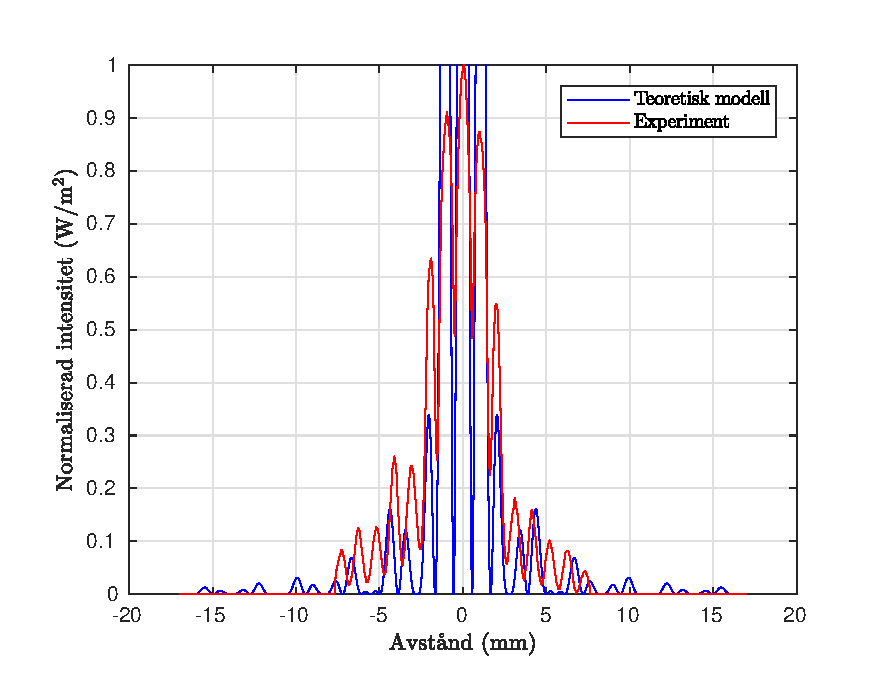
\includegraphics[width=0.75\linewidth]{Data/Figurer/dubbelspalt.eps}
	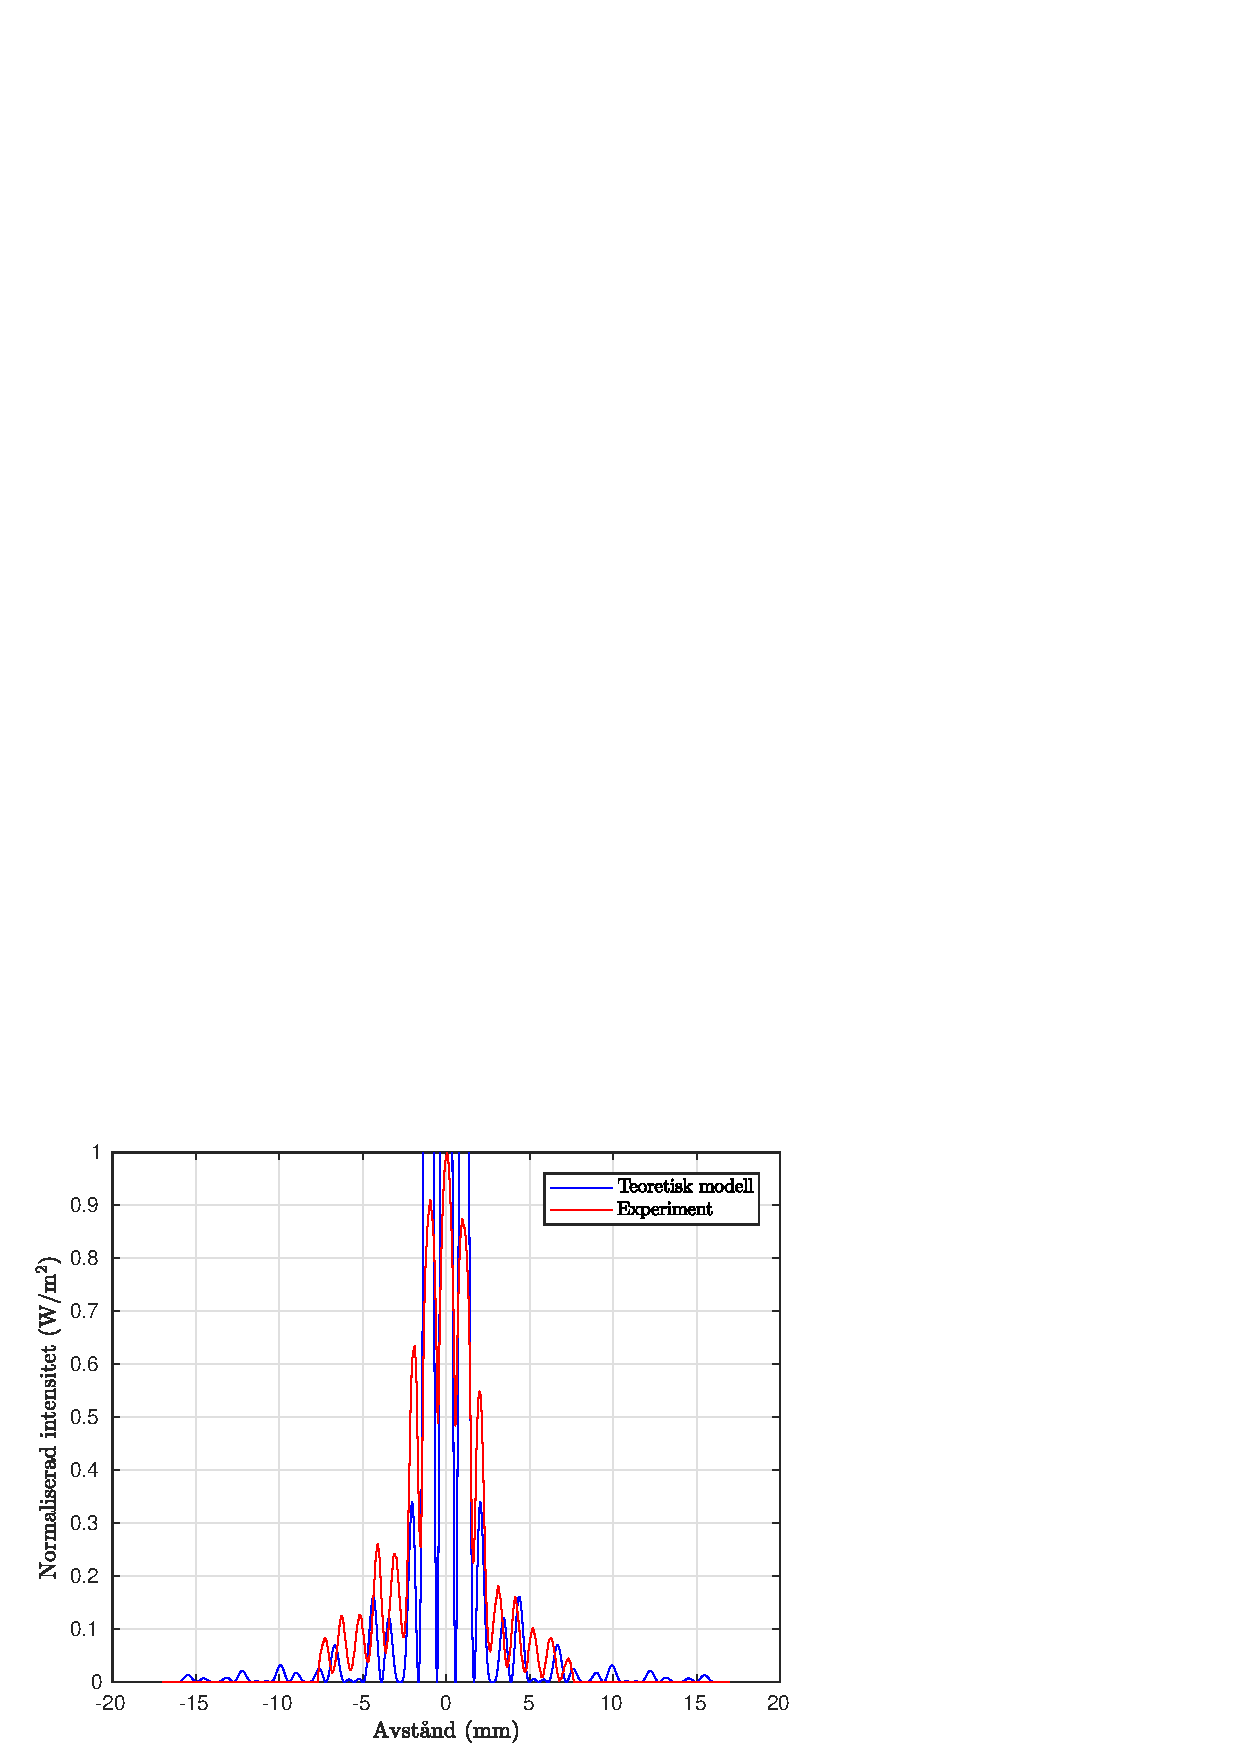
\includegraphics[width=0.5\linewidth]{Data/Figurer/dubbelspalt.png}
	\caption{Interferensmönstret för ett dubbelspaltssystem i Fraunhoferregimen. I figuren visas den experimentella och teoretiska intensitetsfördlningen på ett CCD-chip. Mätningen gjordes med spaltavståndet \SI{250}{\micro\meter} och spaltbredden \SI{100}{\micro\meter}. Avståndet mellan dubbelspalten och skärmen bestämdes till \SI{686}{\milli\meter}.}
	\label{fig:dubbelspalt}
\end{figure}

\FloatBarrier

Efter att avståndet till spalten  bestämts, kunde detta användas för att bestämma spaltavståndet i ett fyrspaltssystem. \autoref{fig:4spalt} visar den experimentella och teoretiska intensitetsfördelningen i Fraunhoferregimen för detta system. Spaltbredden var \SI{77.229}{\micro\m} och spaltavståndet bestämdes till \SI{254.28}{\micro\m}.

\FloatBarrier

\begin{figure}[h!]
	\centering
	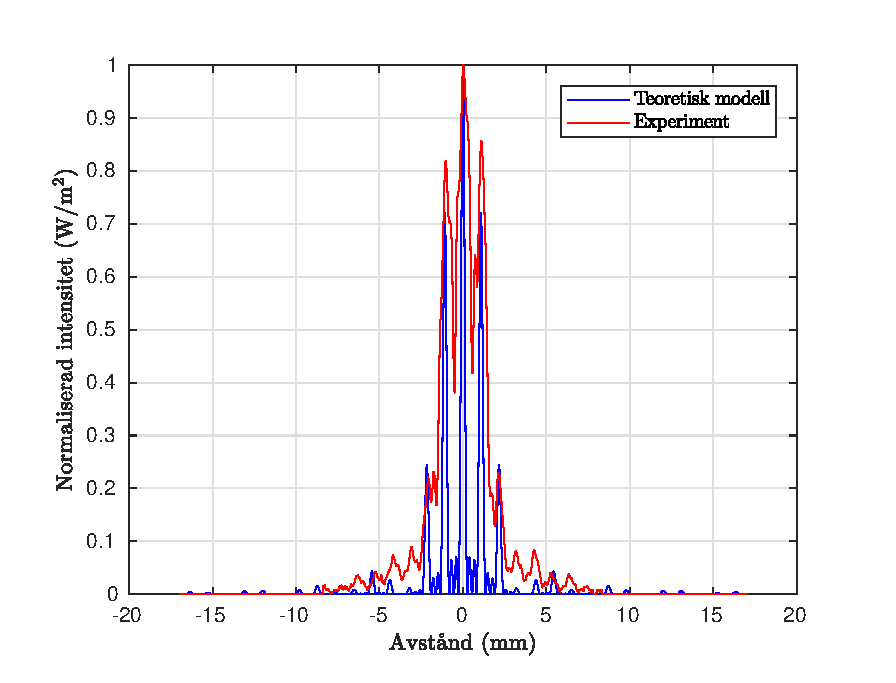
\includegraphics[width=0.75\linewidth]{Data/Figurer/4spalt.eps}
	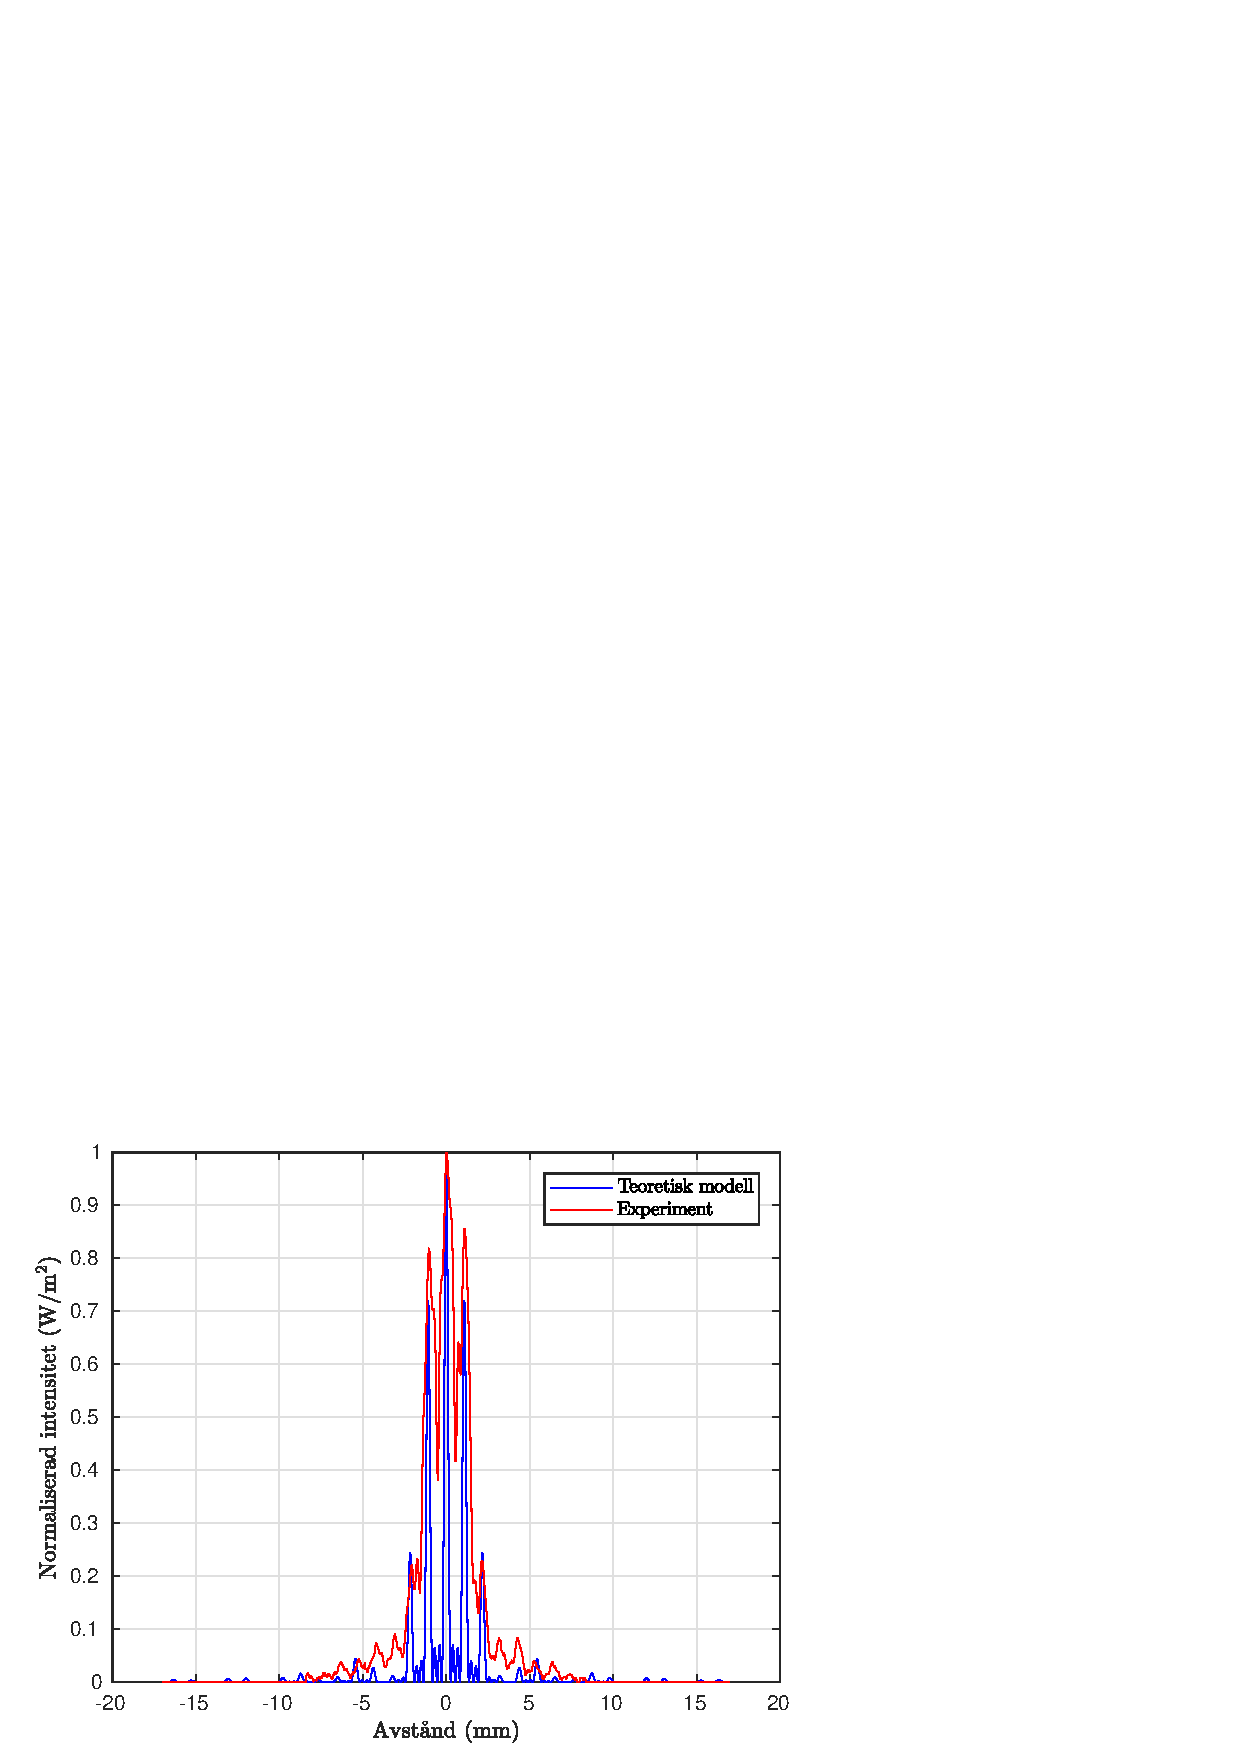
\includegraphics[width=0.5\linewidth]{Data/Figurer/4spalt.png}
	\caption{Den experimentella och teoretiska intensitetsfördlningen på ett CCD-chip för ett fyrspaltssystem. Mätningen gjordes i Fraunhoferregimen med spaltbredden \SI{77.229}{\micro\meter} och spaltavståndet bestämdes till \SI{254.28}{\micro \meter}.}
	\label{fig:4spalt}
\end{figure}

\FloatBarrier

Samma mätning upprepades sedan för en enkelspalt. \autoref{fig:enkelspalt} presenterar den teoretiska och experimentella intensitetsfördelningen I Fraunhoferregimen för denna enkelspalt, varefter spaltbredden bestämdes till \SI{212.22}{\micro\m}.

\FloatBarrier

\begin{figure}[h!]
	\centering
	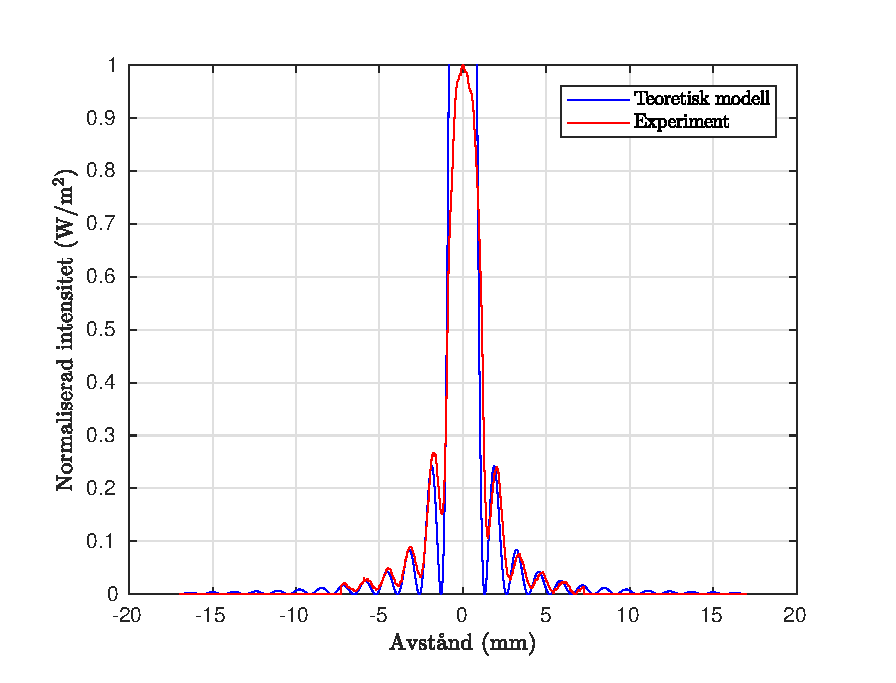
\includegraphics[width=0.75\linewidth]{Data/Figurer/enkelspalt.eps}
	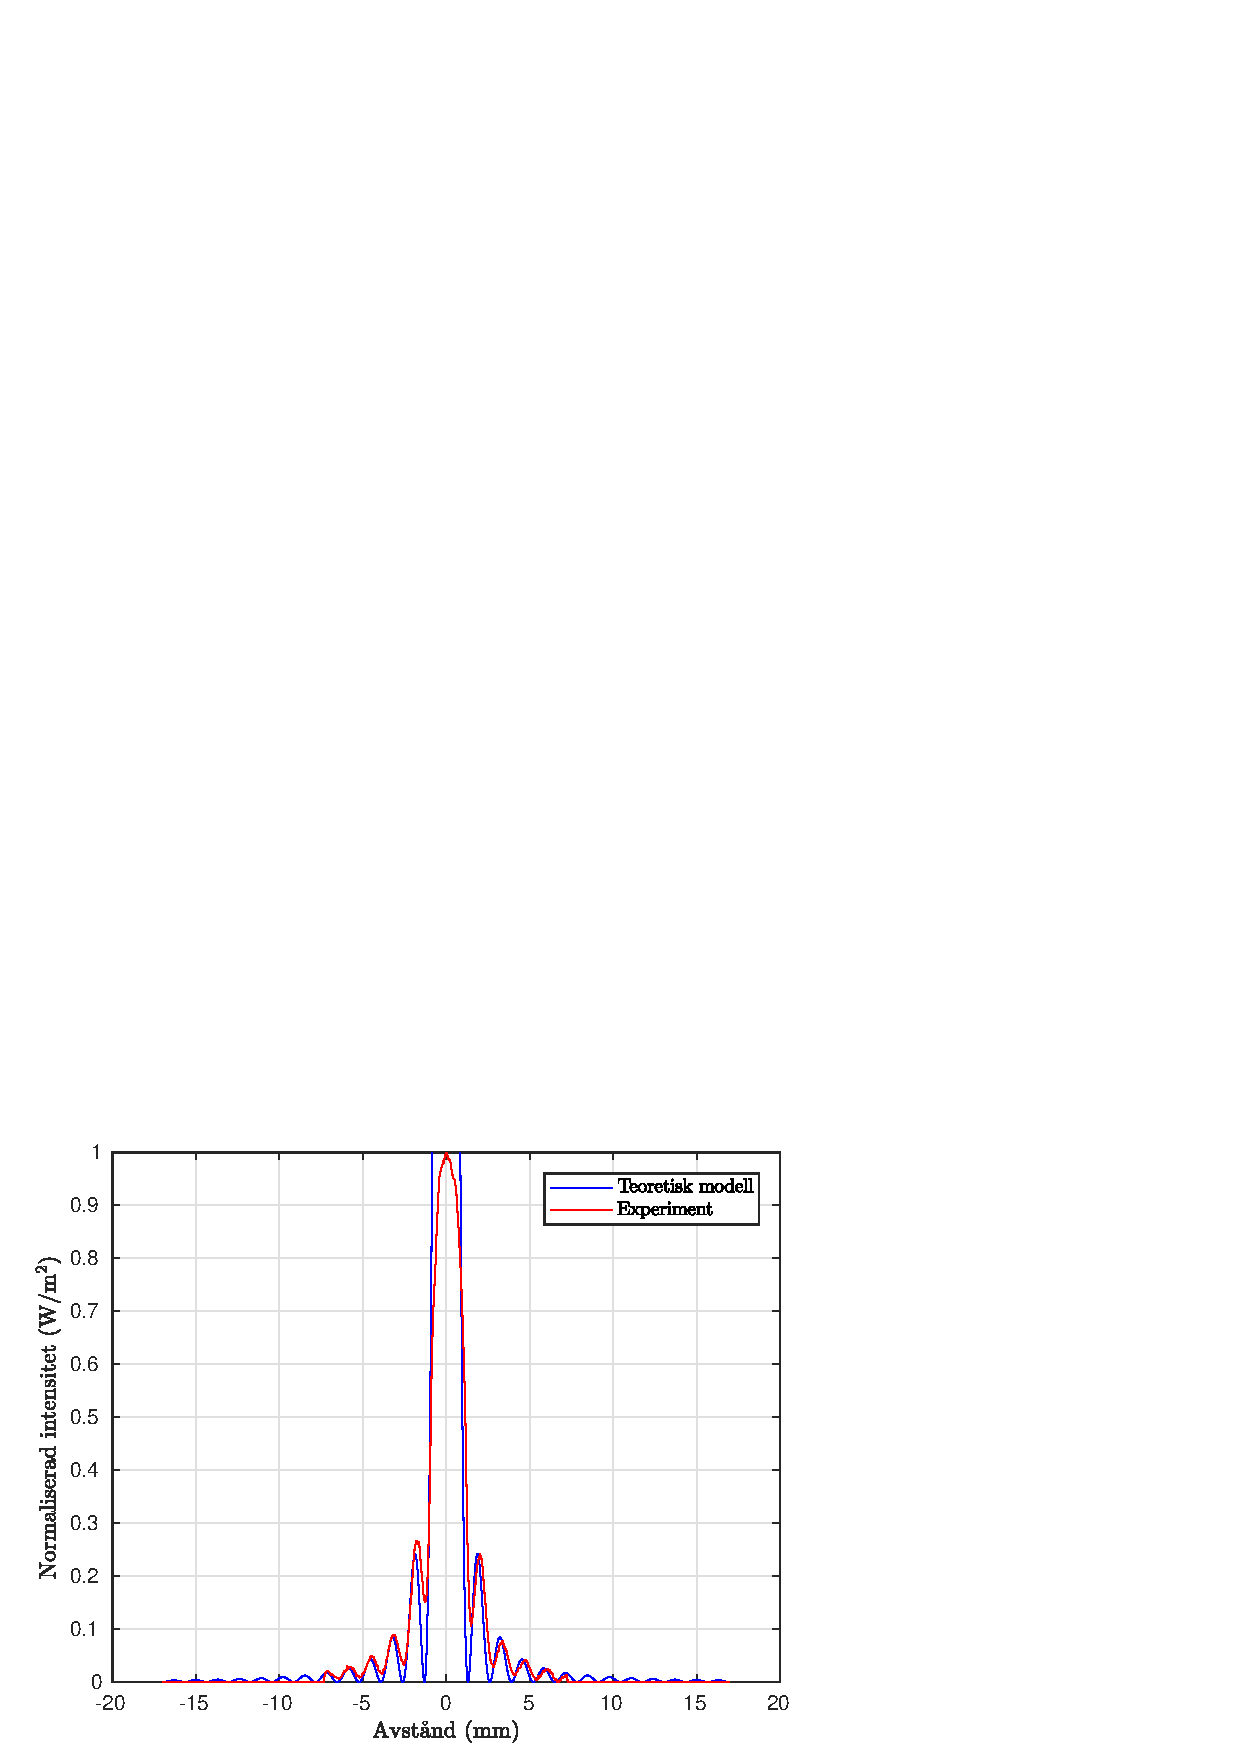
\includegraphics[width=0.5\linewidth]{Data/Figurer/enkelspalt.png}
	\caption{Diffraktionsmönstret för en enkelspalt. Figuren visar den teoretiska och experimentella intensitetsfördelning på ett CCD-chip, där spaltbredden bestämdes till \SI{212.22}{\micro\m}.}
	\label{fig:enkelspalt}
\end{figure}

\FloatBarrier

\autoref{fig:tradHogExpo} och \autoref{fig:tradLagExpo} visar intensitetsfördelningen som uppstår då en tråd med bredden \SI{212.22}{\micro\m} belyses , tillsammans med den teoretiska intensitetsfördelningen av en enkelspalt med samma bredd. I \autoref{fig:tradHogExpo} som är tagen med hög exponering är maxima av högre ordning synliga, medan de lägre är överexponerade. Motsatsen kan ses i \autoref{fig:tradLagExpo} där maxima av ordningen $-1, 0$ och $1$ precis är synliga.

\FloatBarrier

\begin{figure}[h!]
	\centering
	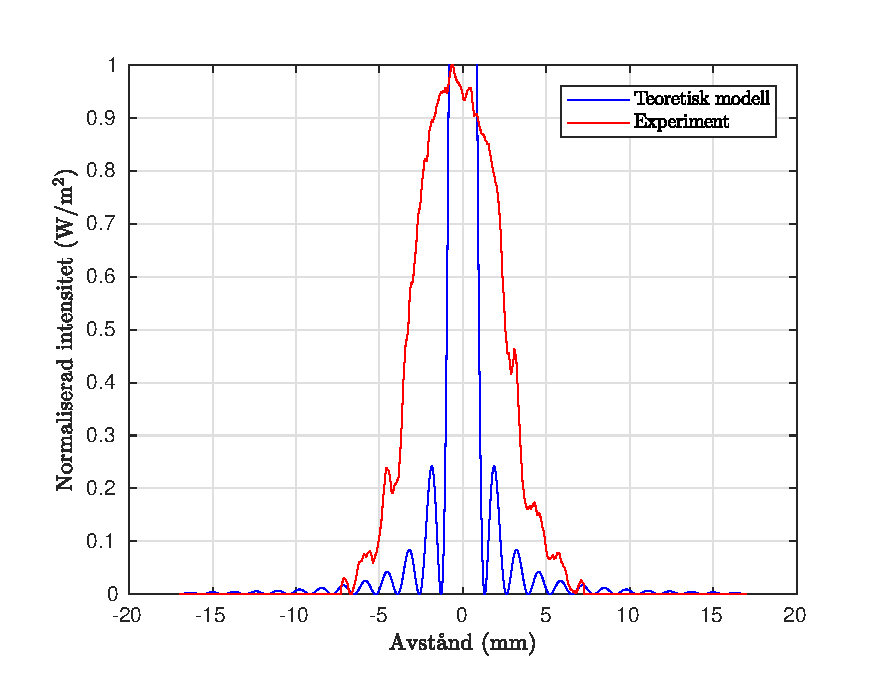
\includegraphics[width=0.75\linewidth]{Data/Figurer/tradHogExpo.eps}
	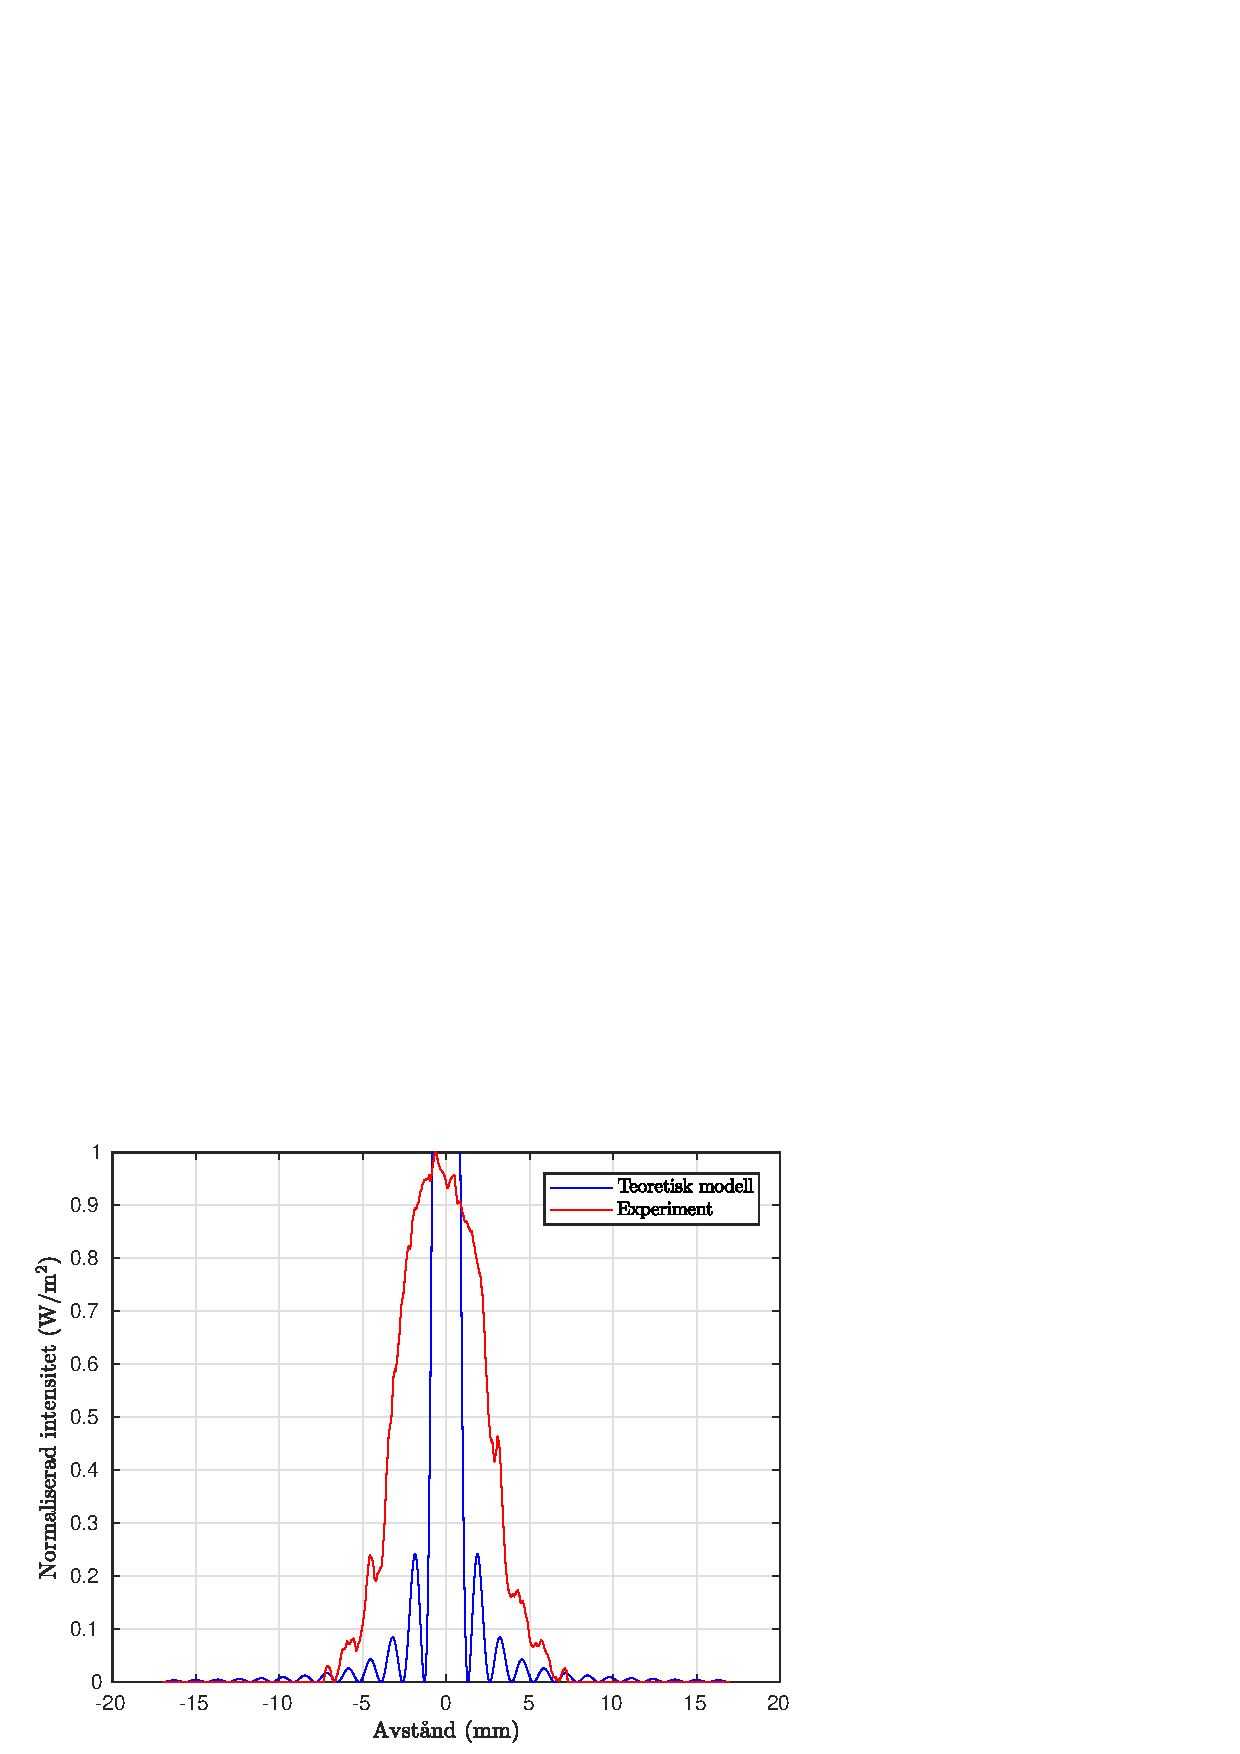
\includegraphics[width=0.5\linewidth]{Data/Figurer/tradHogExpo.png}
	\caption{Diffraktionsmönstret för en tråd med bredden \SI{212.22}{\micro\m}. Bilden togs med hög exponering och i figuren är maxima av högre ordning synliga. Mätningen ritas här tillsammans med diffraktionsmönstret från en enkelspalt med samma bredd.}
	\label{fig:tradHogExpo}
\end{figure}

\begin{figure}[h!]
	\centering
	\includegraphics[width=0.75\linewidth]{Data/Figurer/tradLagExpo.eps}
	\includegraphics[width=0.5\linewidth]{Data/Figurer/tradLagExpo.png}
	\caption{Diffraktionsmönstret för en tråd med bredden \SI{212.22}{\micro\m}. Bilden togs med låg exponering och i figuren är maxima av ordningarna $-1, 0$ och $1$ synliga. Mätningen ritas här tillsammans med diffraktionsmönstret från en enkelspalt med samma bredd.}
	\label{fig:tradLagExpo}
\end{figure}

\FloatBarrier

Intensitetsfördelningen som uppstår då en enkelspalt med spaltbredden \SI{212.22}{\micro\m} och en tråd av samma bred belyses samtidigt presenteras i \autoref{fig:trad+enkelspalt} tillsammans med den teoretiska intensitetsfördelningen av en enkelspalt med samma bredd. Genom mitten av interferensmönstret är en mörk region med låg intensitet syndlig, i både horisontal- och vertikalled.

\FloatBarrier

\begin{figure}[h!]
	\centering
	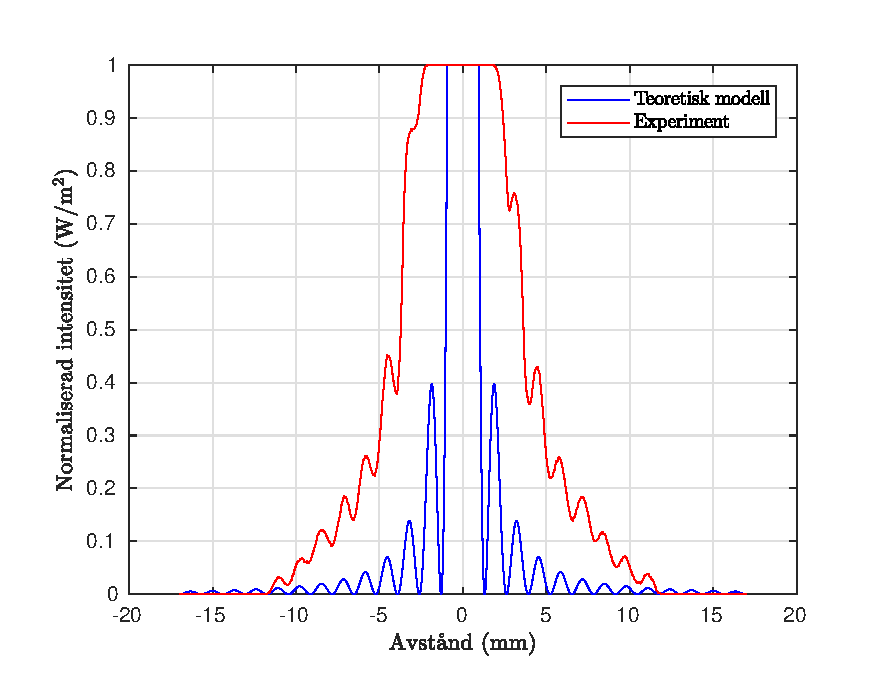
\includegraphics[width=0.75\linewidth]{Data/Figurer/trad+enkelspalt.eps}
	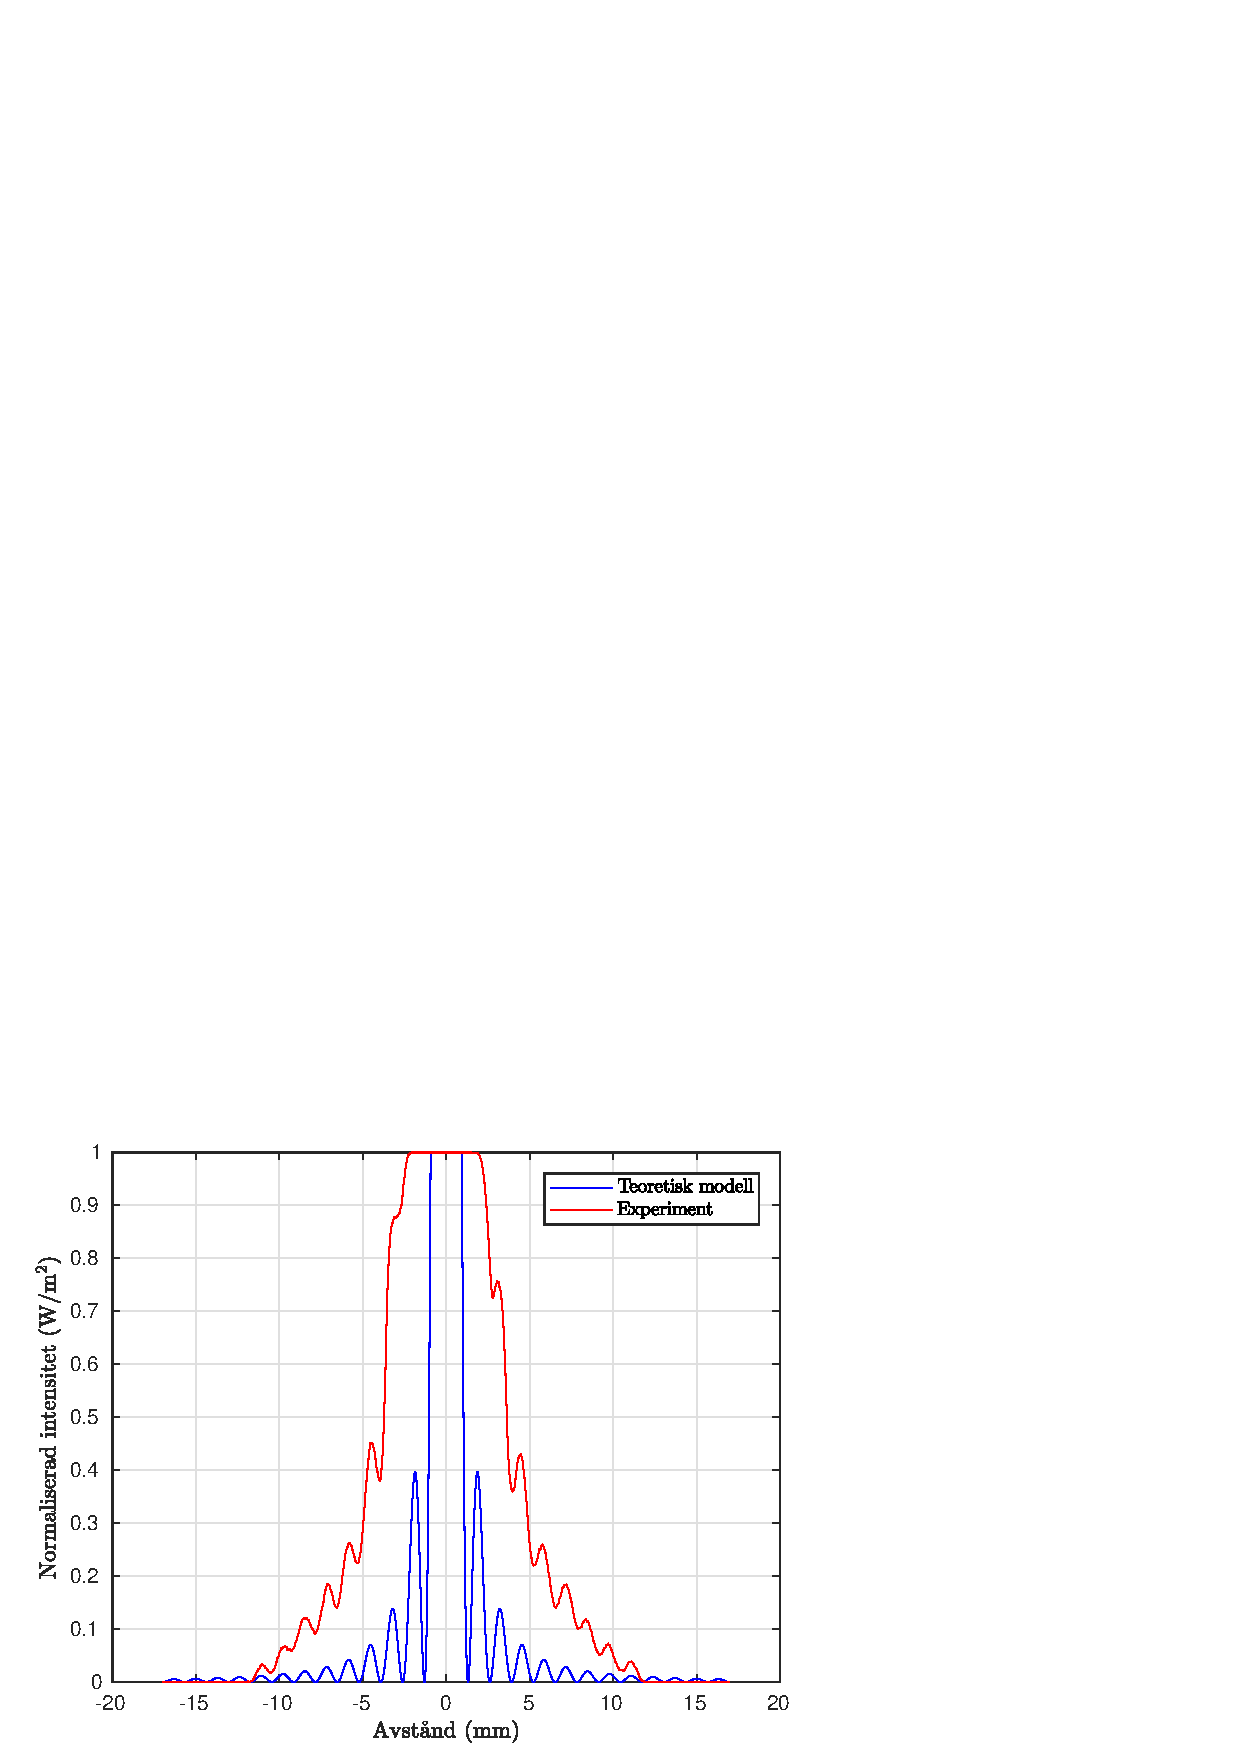
\includegraphics[width=0.5\linewidth]{Data/Figurer/trad+enkelspalt.png}
	\caption{Interferensmönstret då en tråd med bredden \SI{212.22}{\micro\m} och en spalt av samma bredd belyses samtidigt. Genom mitten av mönstret är mörk region med låg intensitet synlig, i både horisontal- och vertikalled.}
	\label{fig:trad+enkelspalt}
\end{figure}

\FloatBarrier

\autoref{fig:variabelEnkelspalt1}, \autoref{fig:variabelEnkelspalt2} och \autoref{fig:variabelEnkelspalt3} visar intensitetsfördelningen i Fraunhoferregimen för en ställbar enkelspalt vid tre olika spaltbredder. För att bestämma spaltbredden justerades denna i den teoretiska intensitetsfördelningen så att mönstren stämmer överens. Detta resulterade i spaltbredderna \SI{153.289}{\micro\m}, \SI{111.2}{\micro\m} och \SI{69.5}{\micro\m}

\FloatBarrier

\begin{figure}[h!]
	\centering
	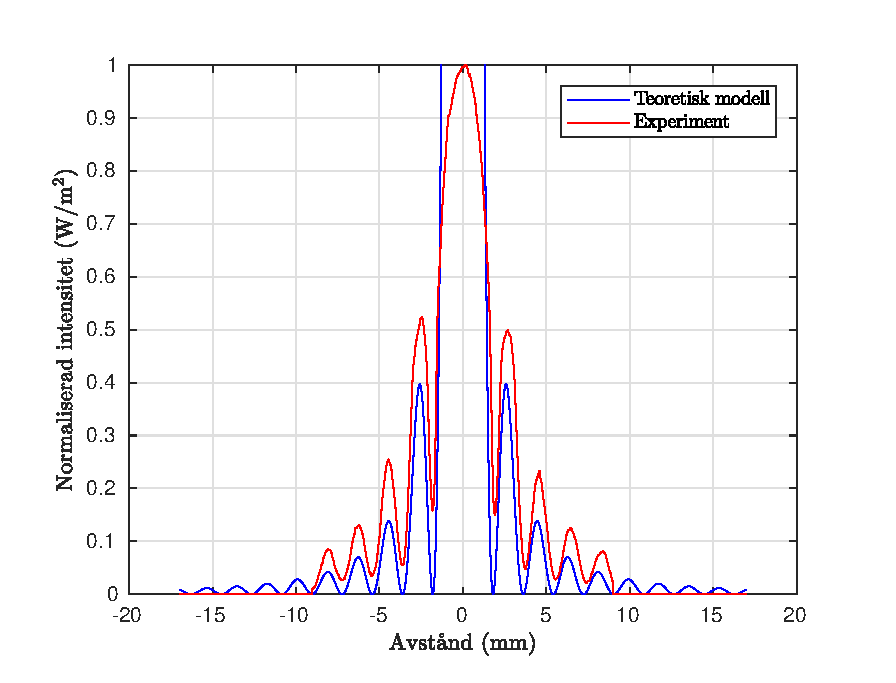
\includegraphics[width=0.75\linewidth]{Data/Figurer/variabelEnkelspalt1.eps}
	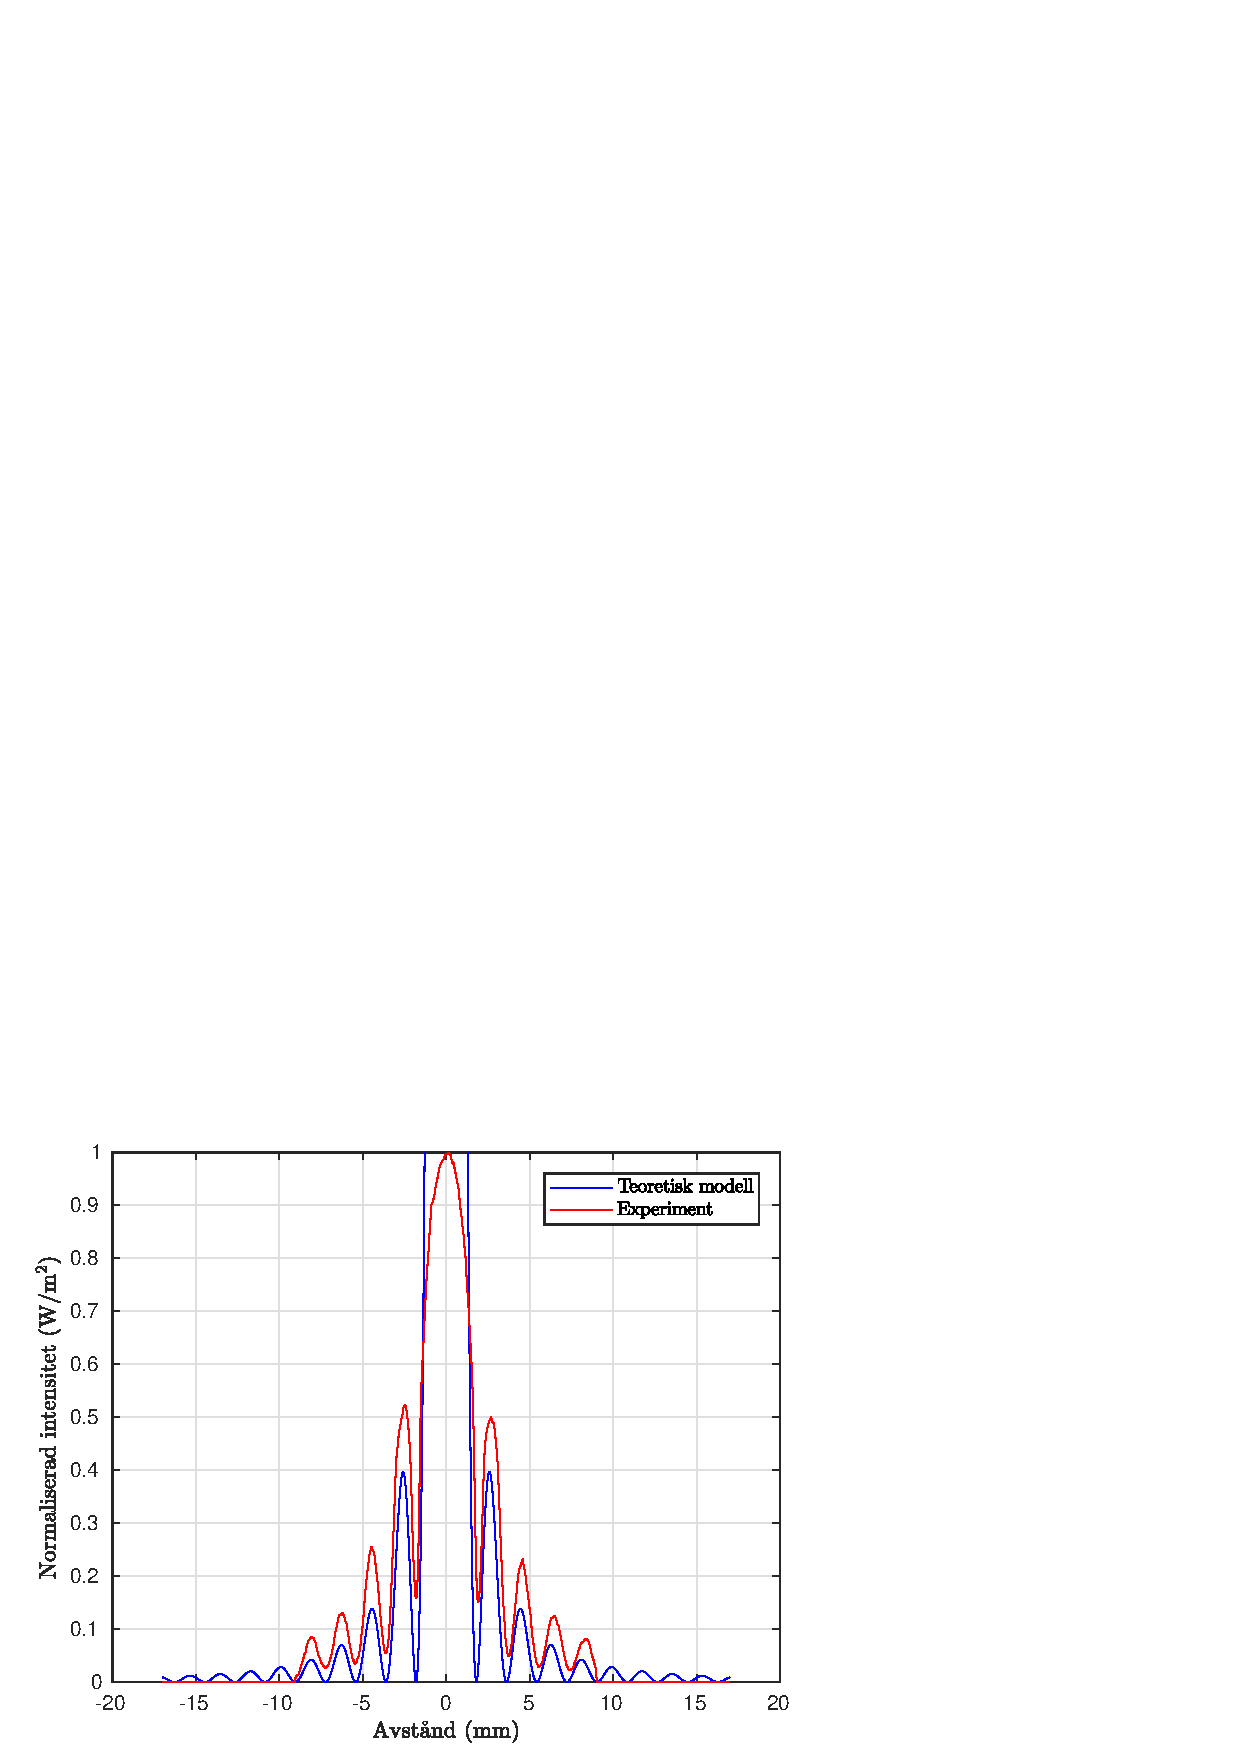
\includegraphics[width=0.5\linewidth]{Data/Figurer/variabelEnkelspalt1.png}
	\caption{Intensitetsfördelningen i Fraunhoferregimen för en variabel enkelspalt med spaltbredden \SI{153.289}{\micro\m}.}
	\label{fig:variabelEnkelspalt1}
\end{figure}

\begin{figure}[h!]
	\centering
	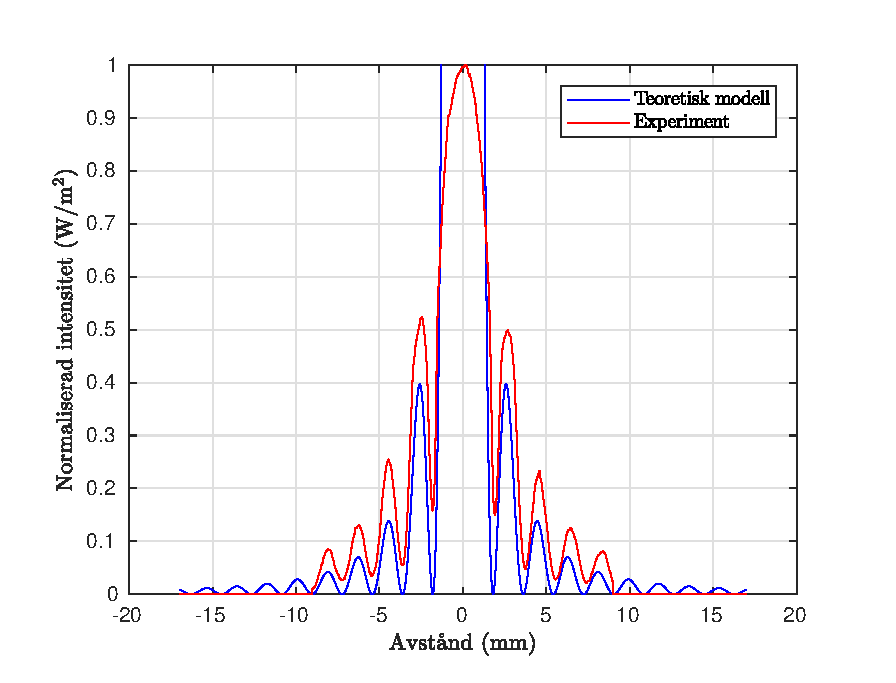
\includegraphics[width=0.75\linewidth]{Data/Figurer/variabelEnkelspalt1.eps}
	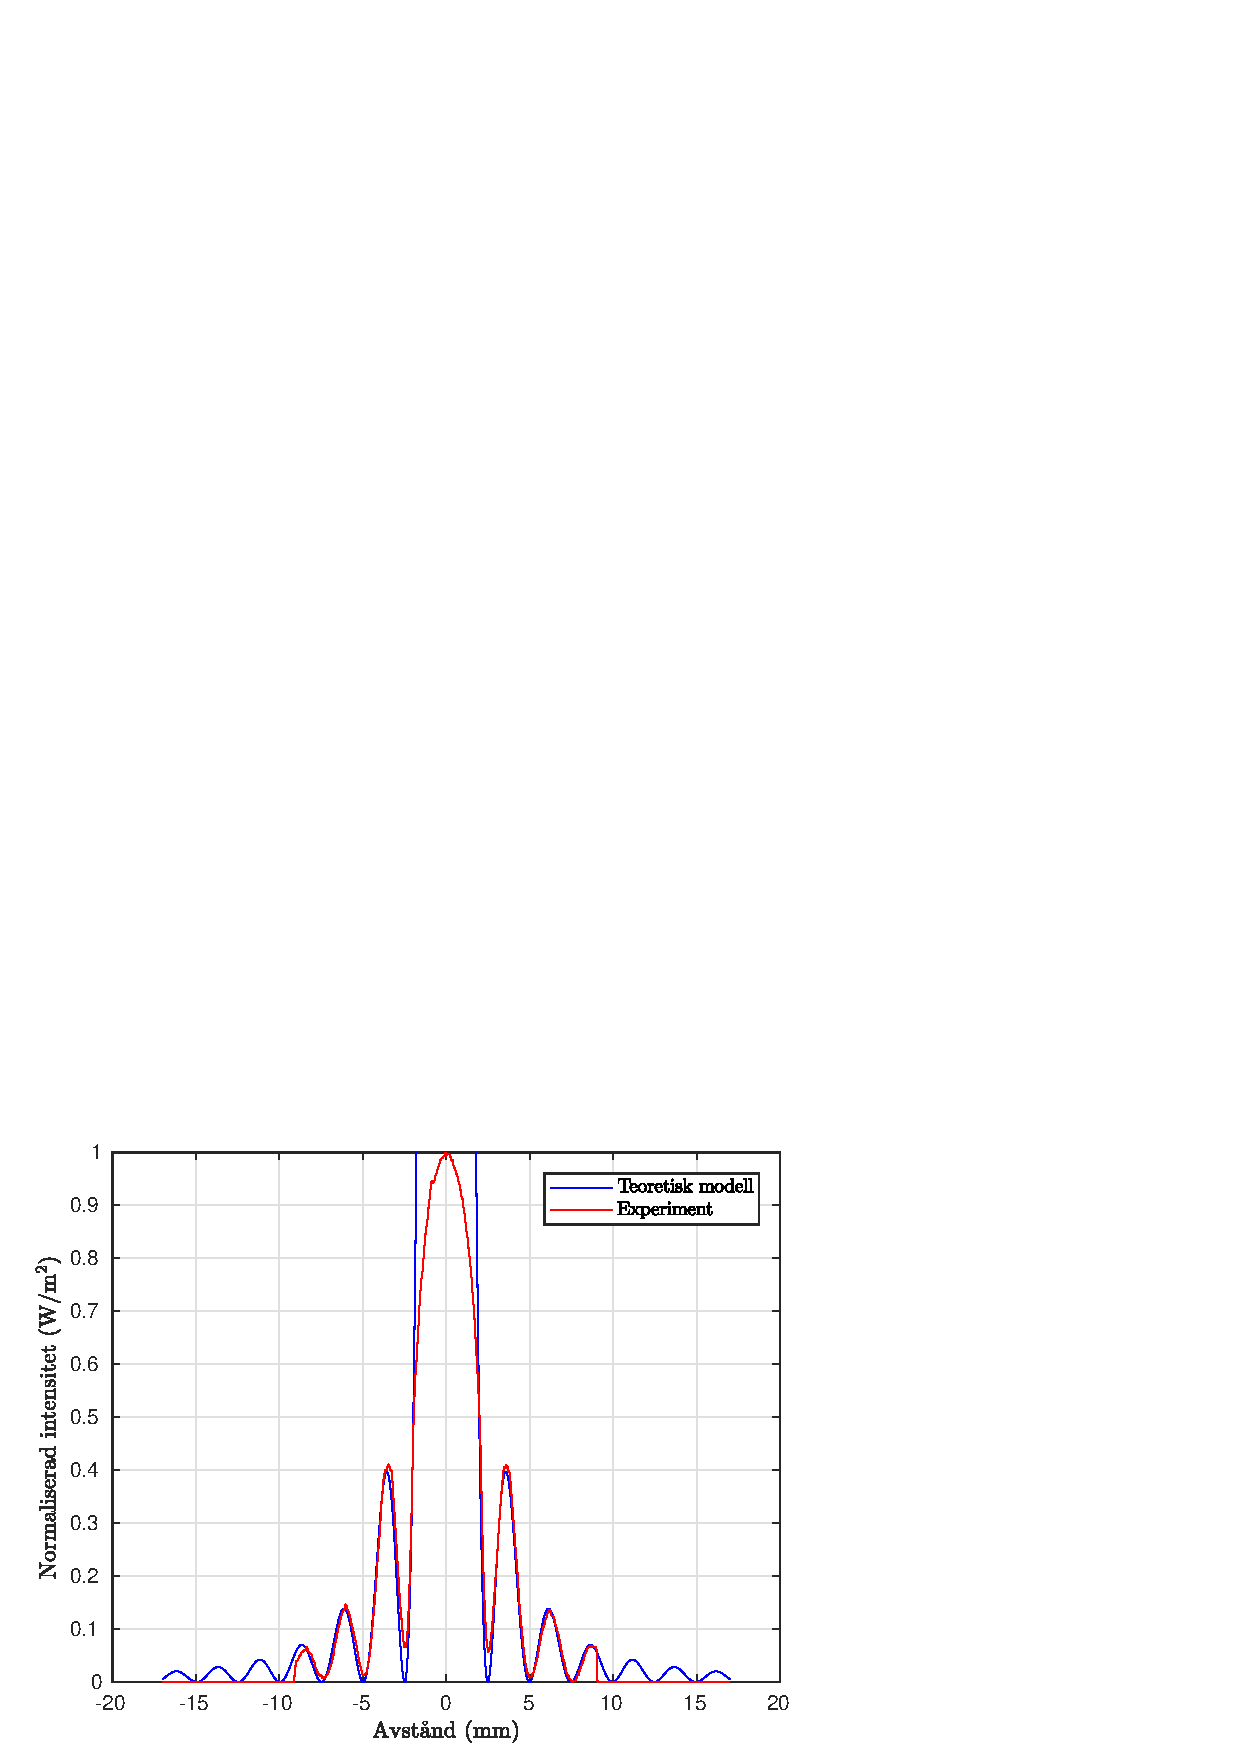
\includegraphics[width=0.5\linewidth]{Data/Figurer/variabelEnkelspalt2.png}
	\caption{Intensitetsfördelningen i Fraunhoferregimen för en variabel enkelspalt med spaltbredden \SI{111.2}{\micro\m}.}
	\label{fig:variabelEnkelspalt2}
\end{figure}

\begin{figure}[h!]
	\centering
	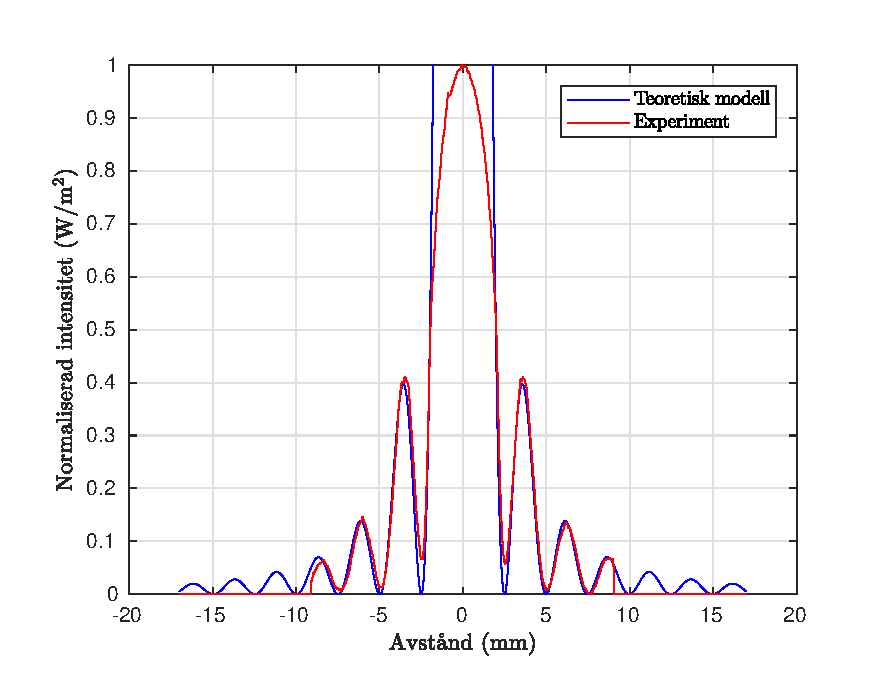
\includegraphics[width=0.75\linewidth]{Data/Figurer/variabelEnkelspalt2.eps}
	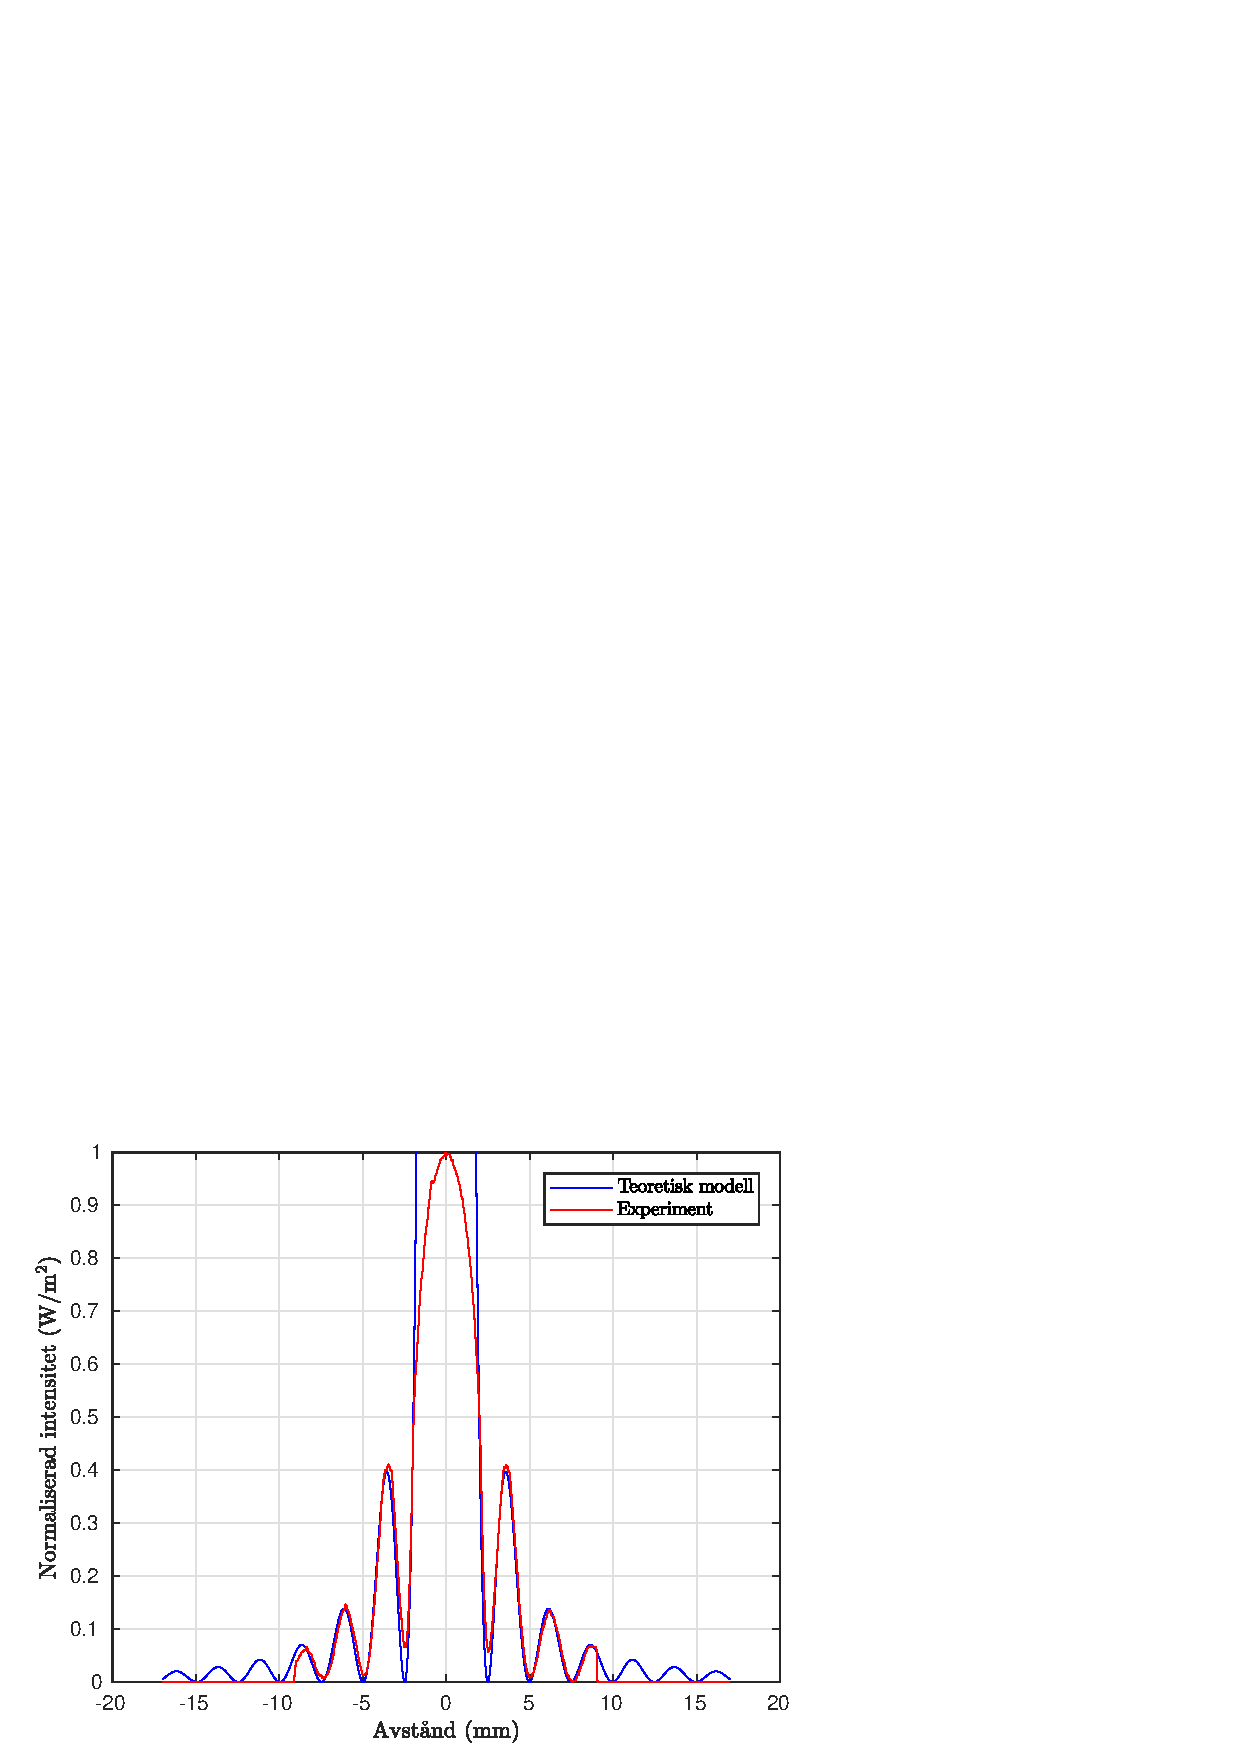
\includegraphics[width=0.5\linewidth]{Data/Figurer/variabelEnkelspalt2.png}
	\caption{Intensitetsfördelningen i Fraunhoferregimen för en variabel enkelspalt med spaltbredden \SI{69.5}{\micro\m}.}
	\label{fig:variabelEnkelspalt3}
\end{figure}

\FloatBarrier

\subsection{Mätning av intensitetsfördelningi Fresnelregimen}

Diffraktionen från en knivegg presenteras i \autoref{fig:edge}. I figuren syns ett tydlig spaltmönster som avtar i intensitet med avståndet från kniveggen.

\FloatBarrier

\begin{figure}[h!]
	\centering
	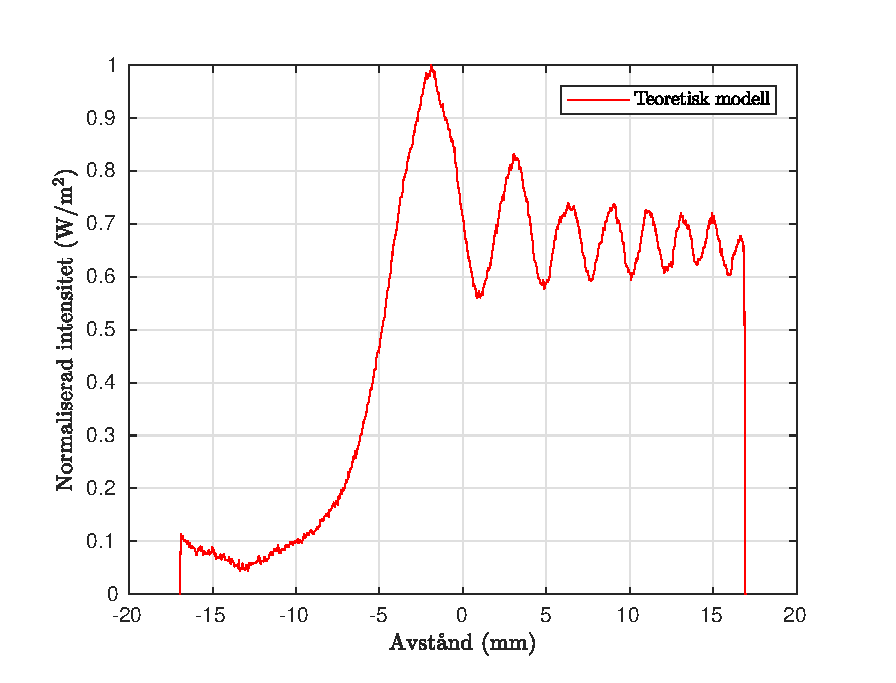
\includegraphics[width=0.75\linewidth]{Data/Figurer/edge.eps}
	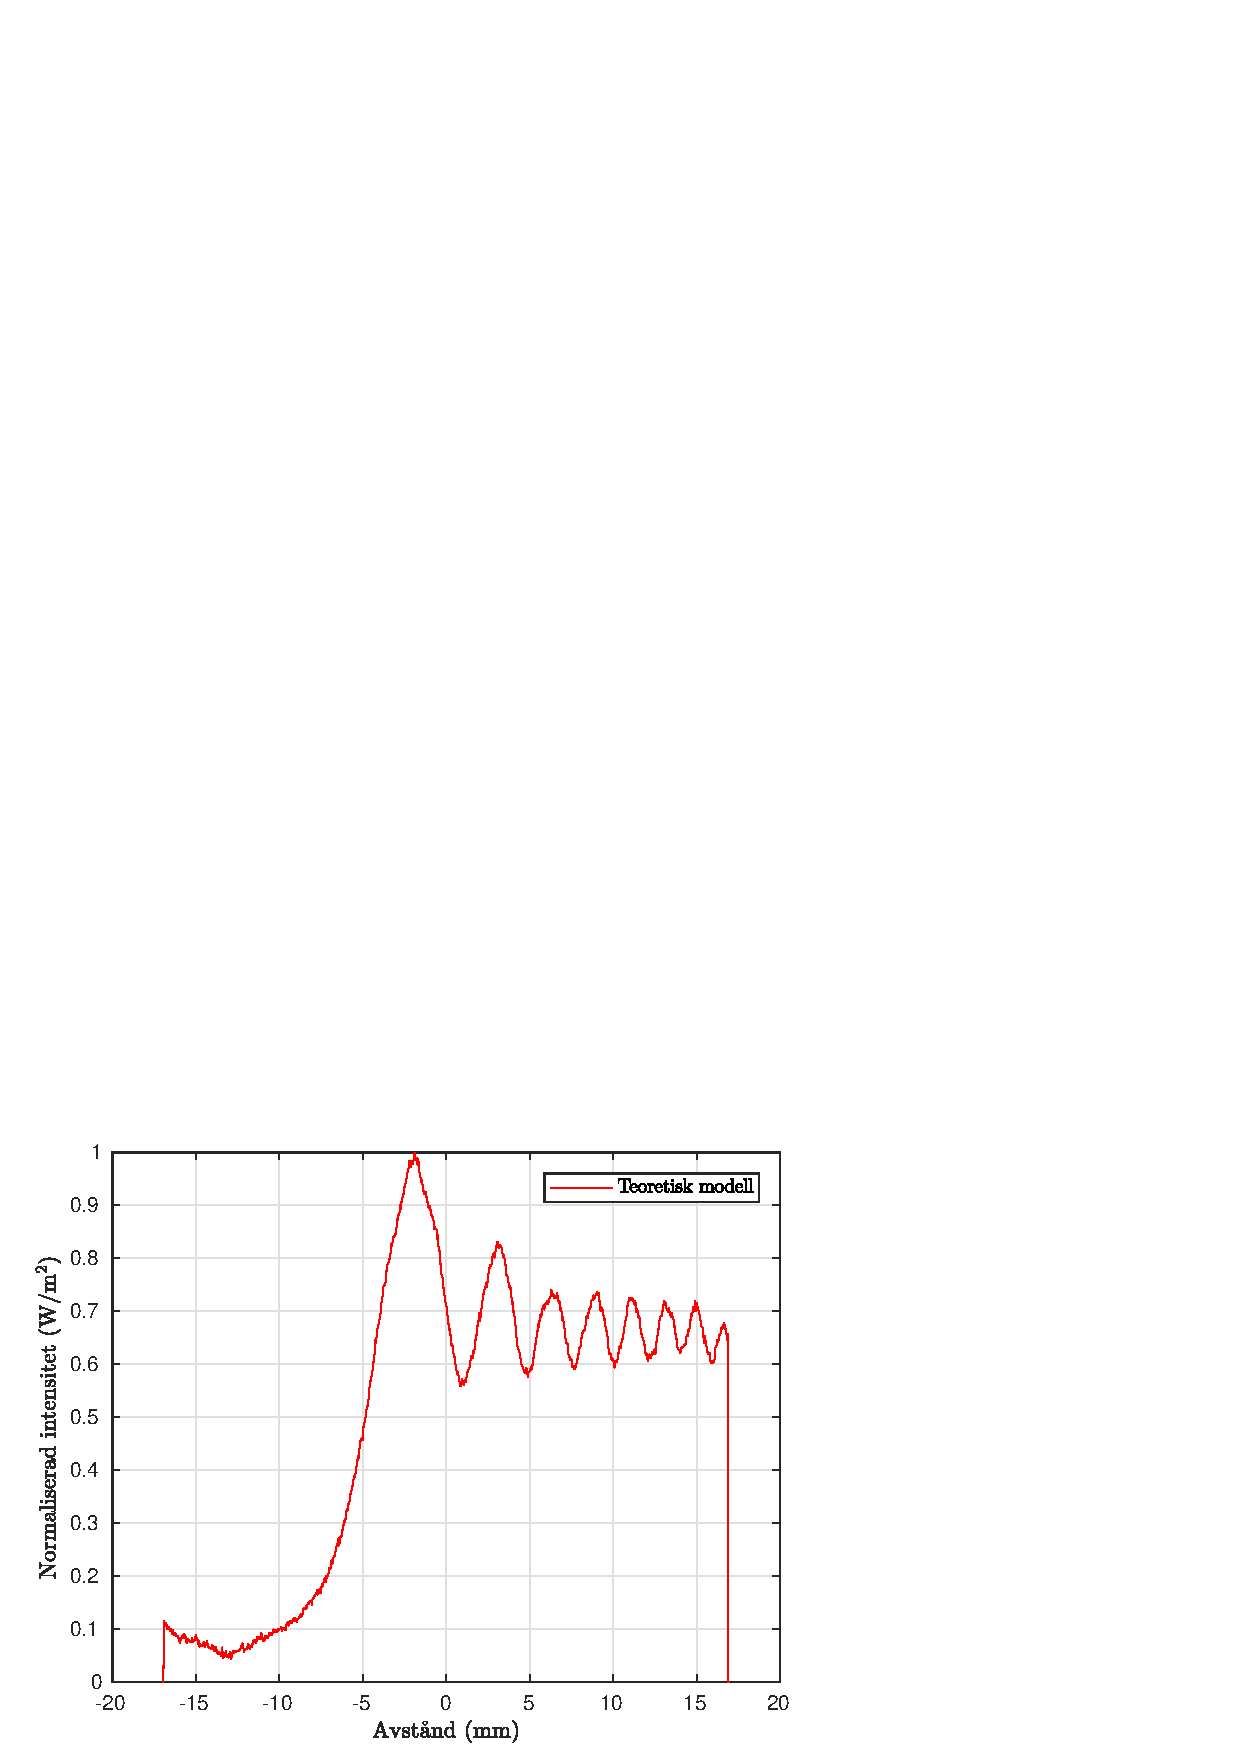
\includegraphics[width=0.5\linewidth]{Data/Figurer/edge.png}
	\caption{Den teoretiska och experimentella intensitetsfördelningen för ljus som belyser en knivegg.}
	\label{fig:edge}
\end{figure}

\FloatBarrier

\autoref{fig:fresnelEnkel} visar en bildsekvens på hur diffraktionsmönstret i Fresnelregimen ändras för minskad spaltbredd, där spaltbredden minskar från vänster till höger. I den sista bilden ses ett mönster mer like Fraunhoferdiffraktion.

\FloatBarrier

\begin{figure}[h!]
	\centering
	\includegraphics[width=0.24\linewidth]{Data/Figurer/fresnelEnkel1.png}
	\includegraphics[width=0.24\linewidth]{Data/Figurer/fresnelEnkel2.png}
	\includegraphics[width=0.24\linewidth]{Data/Figurer/fresnelEnkel3.png}
	\includegraphics[width=0.24\linewidth]{Data/Figurer/fresnelEnkel4.png}
	\caption{Diffraktionsmönster för en variabel enkelspalt i Fresnelregmien. Spaltbredden minskar från vänster till höger.}
	\label{fig:fresnelEnkel}
\end{figure}

\FloatBarrier

\subsection{Datorsimuleringar}

\section{Diskussion}
  %Är resultaten rimliga? Vad hade kunnat göras annorlunda?

\section{Slutsats}
  %En   sammanfattning  där   man  till   skillnad  från   den  inledande
  %sammanfattningen förutsätter  att läsaren har läst  rapporten, samt de
  %slutsatser man kan dra av det gjorda arbetet.
 
 \bibliography{bibliography}{}
 \bibliographystyle{plain}

\end{document}
